\section{Processing of a Single Subject-Verb Dependency in the Italian NLM}\label{single_dependency_Italian}
We focus here on Italian instead of English for three main reasons. First, we aimed to replicate the English results on another language. Second, the Italian NLM made available by \citet{Gulordava:etal:2018} achieves better performance than the English NLM on nested constructions, which are computationally more demanding compared to sentences in the NounPP NA-task explored in \citet{lakretz2019emergence}, and which will constitute the main object of our study. This might be explained by the fact that Italian is morpho-syntactically richer than English, making it more important for the NLM to pick up grammatical information. Third, in English, the plural is identical to the unmarked form of the verb, which can occur as infinitive, in first and second person, and often as a noun. This makes the occurrence statistics extremely unbalanced in favor of plural.\footnote{\citet{Gulordava:etal:2018} made available models in English, Italian, Hebrew and Russian, which were optimized by conducting a grid search on the language modeling objective, and became since a subject of research in several subsequent studies \citep{Giulianelli:etal:2018, jumelet2019analysing, wilcox2018rnn, futrell2019neural}. We directly use their model without any further tuning.}

Furthermore, agreement in Italian can also occur with respect to gender, for instance, in sentences containing predicative adjectives: ``il \textbf{bambino} accanto alla \underline{madre} \`{e} \textbf{bello}'' (``The (m.) \textbf{boy} near the (f.) \underline{mother} is pretty (m.)''), in which subject and predicate agree with respect to both number and gender. This allowed us to test whether the previous results in English hold for another grammatical feature. We therefore hypothesize that there should also exist long-range `gender' units in the network, with dynamics that are robust to possible attractors (e.g., to ``madre'' above, which is feminine). To test this and whether the Italian NLM has developed agreement mechanism for number, similar to the model trained on English, we followed the same steps described in the previous section--an ablation study, visualization of unit dynamics and a connectivity analysis.\footnote{Due to lack of relevant resources, we do not attempt to track down syntax units. The very fact that the Italian NLM handles various long-distance agreement tasks correctly, as shown here and in the next section, suggests that similar units must control the dynamics of its long-range number units. Proving their presence is in any case not crucial to our main predictions.}


\subsection{Methods and Materials}
\subsubsection{Agreement Tasks}
For the ablation studies, we constructed two \emph{agreement tasks} with a single long-range dependency across a prepositional phrase \citep{lakretz2019emergence}: NounPP-number and NounPP-gender. In the NounPP-number task, the main subject and verb agree on grammatical number, and a second noun (attractor) can interfere during sentence processing. This task was used to identify long-range number units. The NounPP-gender task, the main subject and a predicative adjective agree on gender, and an attractor having an opposite gender can interfere in the middle. This task was used To identify long-range gender units. Table~\ref{tab:na-tasks-overview} (top) describes the two tasks.

\begin{table}[h]
    \setlength\tabcolsep{3mm}
\small
\centering
\begin{tabular}{lll}
\multicolumn{3}{c}{\centering \textit{Agreement tasks for ablation experiments}}\\
\hline
\hline
\emph{NounPP-number} & \texttt{\textbf{NP$_a$} prep NP$_b$ \emph{V$_a$}} & \specialcell{Il \textbf{ragazzo} accanto alla \underline{donna} \textbf{conosce}\vspace{-1mm}\\({\scriptsize The \textbf{boy} next to the \underline{woman} \emph{knows}})} \\
\emph{NounPP-gender} & \texttt{\textbf{NP$_a$} prep NP$_b$ BE$_a$ \emph{ADJ$_a$}} & \specialcell{Il \textbf{ragazzo} accanto alla \underline{donna} \`{e} \textbf{basso}\vspace{-1mm}\\({\scriptsize The \textbf{boy} next to the \underline{woman} is \textbf{short-m}})}\\
\vspace{-2mm}\\
\multicolumn{3}{c}{\centering \textit{Number-agreement tasks for nesting experiments}}\\
\hline
\hline
\emph{Short-Successive} & \texttt{NP$_a$ V$_a$ che NP$_b$ V$_b$} & \specialcell{Il \textbf{figlio} \textbf{dice} che il \emph{ragazzo} \emph{ama}\vspace{-1mm}\\{\scriptsize The \textbf{son} \textbf{says} that the \emph{boy} \emph{loves}}} \\
\emph{Long-Successive} & \texttt{NP$_a$ V$_a$ che NP$_b$ P NP$_c$ V$_b$} & \specialcell{Il \textbf{figlio dice} che l'\emph{amico} accanto al \underline{ragazzo} \emph{conosce}\vspace{-1mm}\\{\scriptsize The \textbf{son says} that the \emph{friend} next to the \underline{boy} \emph{knows}}} \\
\emph{Short-Nested} & \texttt{NP$_a$ che NP$_b$ V$_b$ V$_a$ } & \specialcell{Il \textbf{figlio} che il \emph{ragazzo} \emph{osserva} \textbf{evita}\vspace{-1mm}\\{\scriptsize The \textbf{son} that the \emph{boy} \emph{observes} \textbf{avoids}}} \\
\emph{Long-Nested} & \texttt{NP$_a$ che NP$_b$ P NP$_c$ V$_b$ V$_a$} & \specialcell{Il \textbf{figlio} che la \emph{ragazza} accanto ai \underline{padri} \emph{ama} \textbf{evita}\vspace{-1mm}\\{\scriptsize The \textbf{son} that the \emph{girl} next to the \underline{fathers} \emph{loves} \textbf{avoids}}} \\
\end{tabular}
\caption{\textbf{Agreement tasks for the ablation and nesting experiments.}
The first column denotes the name of the task, the second shows the sentence templates, where \texttt{NP} is used as an abbreviation of \texttt{Det N}.
The indices $a$, $b$ mark the subject-verb dependencies in the templates. 
%For example, in \emph{Long-Nested}, there are three nouns and two verbs, the indices $a$ and $b$ indicate that the last verb \texttt{V$_a$} is syntactically dependent on the first noun phrase \texttt{NP$_a$}, whereas the penultimate verb \texttt{V$_b$} instead should match the features of the second noun phrase \texttt{NP$_b$}.
Note that for \emph{Long-} and \emph{Short-Nested}, we test performance on both the \emph{embedded} verb \texttt{V$_b$} and the \emph{main} verb \texttt{V$_a$}.
The last column contains an example of a sentence in the corresponding agreement task, along with its English translation.
Bold and italic face highlight the dependencies marked by the indices in the templates.
For each agreement task, we systematically vary the \emph{number} (or gender, in \emph{NounPP-gender}) of all nouns in the template, resulting in four different conditions (SS, SP, PS and PP) for the number-agreement tasks with two nouns (\emph{NounPP-number}, \emph{NounPP-gender}, \emph{Short-Successive} and \emph{Short-Nested}) and eight different conditions (SSS, SSP, SPS, SPP, PSS, PSP, PPS and PPP) for the number-agreement tasks with three nouns (\emph{Long-Successive} and \emph{Long-Nested}).
The examples shown are all SS and SSS conditions. For  \emph{NounPP-gender}, singular (S) and plural (P) are replaced by feminine and masculine.
\label{tab:na-tasks-overview}}
\end{table}

\subsubsection{Neural Language Models}
In computational linguistics, a \emph{language model} defines a probability distribution over sequences of words. A Neural Language Model (NLM) is simply a language model implemented by a neural network. The recurrent NLM we use here, schematically illustrated in Figure \ref{fig:lstm}, factorizes the probability of a sentence into a multiplication of the conditional probabilities of all words in the sentence, given the words that precede them:

\begin{equation}
    P(w_1 w_2 \cdots w_n) = \prod_i p(w_i|w_1 \cdots w_{i-1})
\end{equation}

This type of language model can thus be used as \emph{next-word predictor}: given the preamble of a sentence, it outputs a probability distribution over potential next words.
We exploit this fact in our experiments.

\begin{figure}
    \centering
    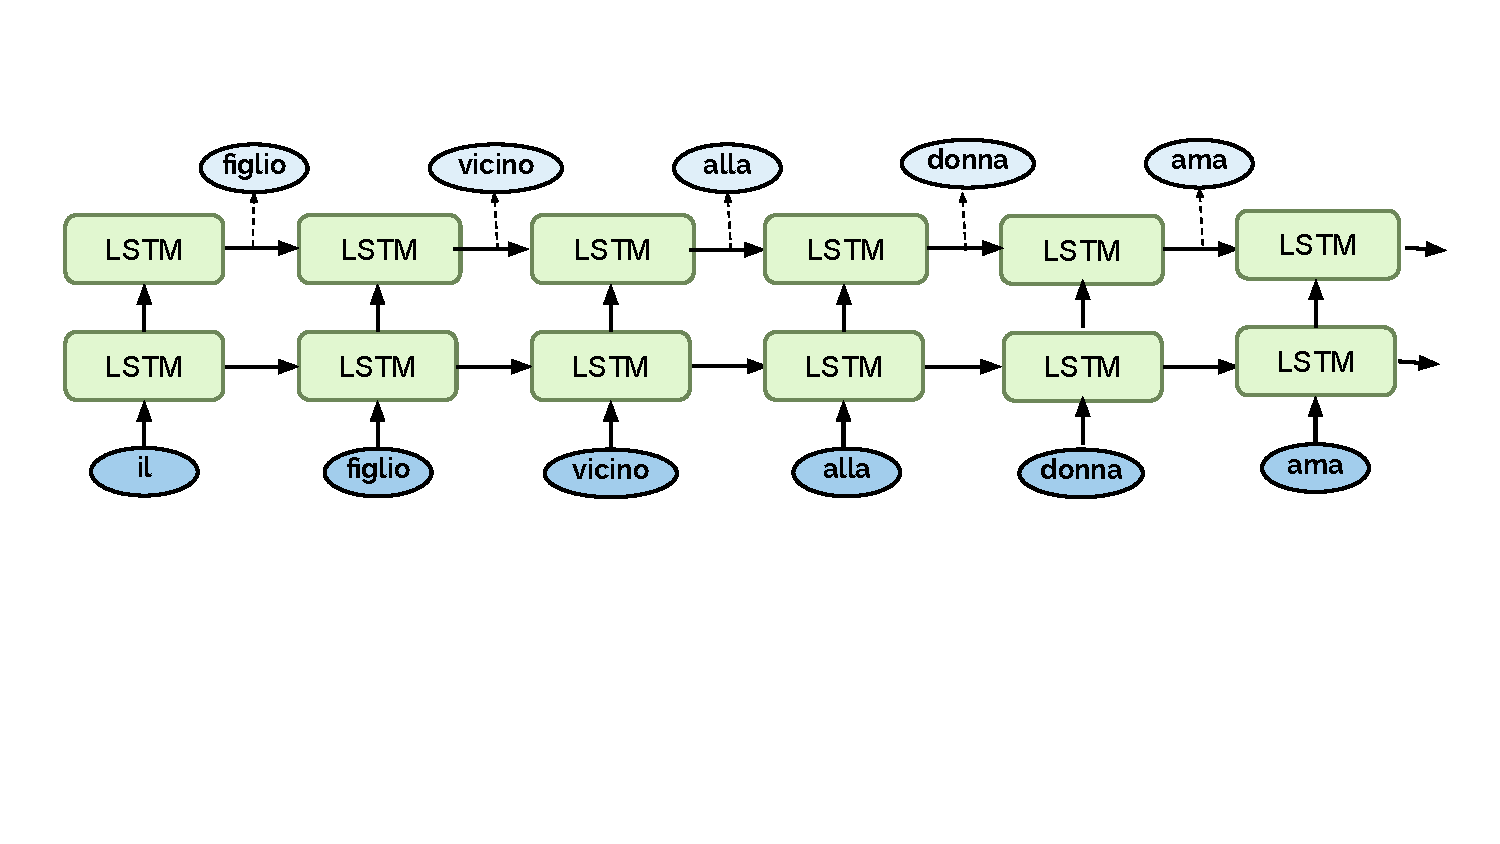
\includegraphics[width=0.8\textwidth, clip, trim={10mm 50mm 10mm 20mm}]{figures/LM-image}
    \caption{Graphical description of a two-layer recurrent neural language model with LSTM cells \citep[not discussed here; see, e.g.,][]{Goldberg:2017}. At each timestep, the model processes an input word and outputs a probability distribution over potential next words in the sentence. The prediction of the output word depends on both the input word and on the previous state of the model, which serves as longer-term context (the horizontal arrows in the figure represent the \emph{recurrent} connections carrying the previous state through).} \label{fig:lstm}
\end{figure}

\subsubsection{Model description}
The specific NLM we used in our experiments is the Italian NLM made available by \citet{Gulordava:etal:2018}\footnote{\url{https://github.com/facebookresearch/colorlessgreenRNNs}}.
It is a recurrent LSTM language model \citep{Graves:2012}, consisting of two layers, each with 650 Long-Short Term Memory units  \citep{Hochreiter:Schmidhuber:1997}, input and output embedding layers of 650 units and input and output layers of size 50000 (the size of the vocabulary). 
The weights of the input and output embedding layers are not shared \citep{press2016using}.
The last layer of the model is a softmax layer, whose activations sum up to 1 and as such corresponds to a probability distribution over all words in the NLM's vocabulary. 

\subsubsection{Model training}
The weights of a NLM are typically tuned by presenting them with large amounts of data (a \emph{training corpus}) and providing them feedback on how well they can predict each next word in the running text. This allows them to adjust their parameters to maximize the probabilities of the sentences in the corpus. %
Our NLM was trained on a sample of the Italian Wikipedia text, containing 80M word tokens and 50K word types. Further details can be found in \citet{Gulordava:etal:2018}.


\subsubsection{Model evaluation on the NA-tasks}\label{sss:model_eval}
Following \citet{Linzen:etal:2016}, we computed the model's accuracy for the different NA-tasks by considering whether the model prefers the correct verb or adjective form (for the NounPP-number and NounPP-gender tasks, respectively) given the context. We did so by presenting the preamble of each sentence to the NLM and then comparing the output probabilities assigned to the plural and singular forms of the verb for the NounPP task and the probabilities of the masculine and feminine forms of the adjective for the NounPP-gender task. On each sentence, the model was scored 1 if the probability of the correct verb (or adjective) was higher than that of the wrong one, and else 0. 
The model's accuracy was then defined as the average of these scores across all sentences in the NA-task. 

\subsubsection{Ablation experiments}
To identify units that play an important role in encoding number or gender, we conducted a series of ablation tests.
In these ablation tests, we assessed the impact of a single unit on model performance by setting the activation of the unit to zero and then recomputing the performance of the model on the NounPP-noun and NounPP-gender NA-tasks. 
We conducted such ablation studies for all recurrent units in the network, resulting in 1300 ablation studies per task.

\subsection{Results}
\subsubsection{Ablation Results Reveal a Long-Range Number Unit} To identify unit(s) that encode grammatical number for long-range dependencies, we conducted an ablation study with the pre-trained Italian model of \citet{Gulordava:etal:2018}, following the steps described above, using an Italian NounPP NA-task. 
We found that the ablation of one unit from the second layer of the network, unit 815, leads to a significant reduction in performance in both incongruent conditions (Figure \ref{fig:ablation_K_model}). For robustness, we repeated the ablation experiment with 19 NLMs that we trained on the same corpus and using the same hyperparameters, varying random initializations only. We found that most models showed a significant reduction in performance after ablation of only a few units, with some models showing a significant effect on the SP or PS condition only, and others on both (Figure \ref{fig:ablation_all_models}).

\begin{figure}[t!]
    \centering
    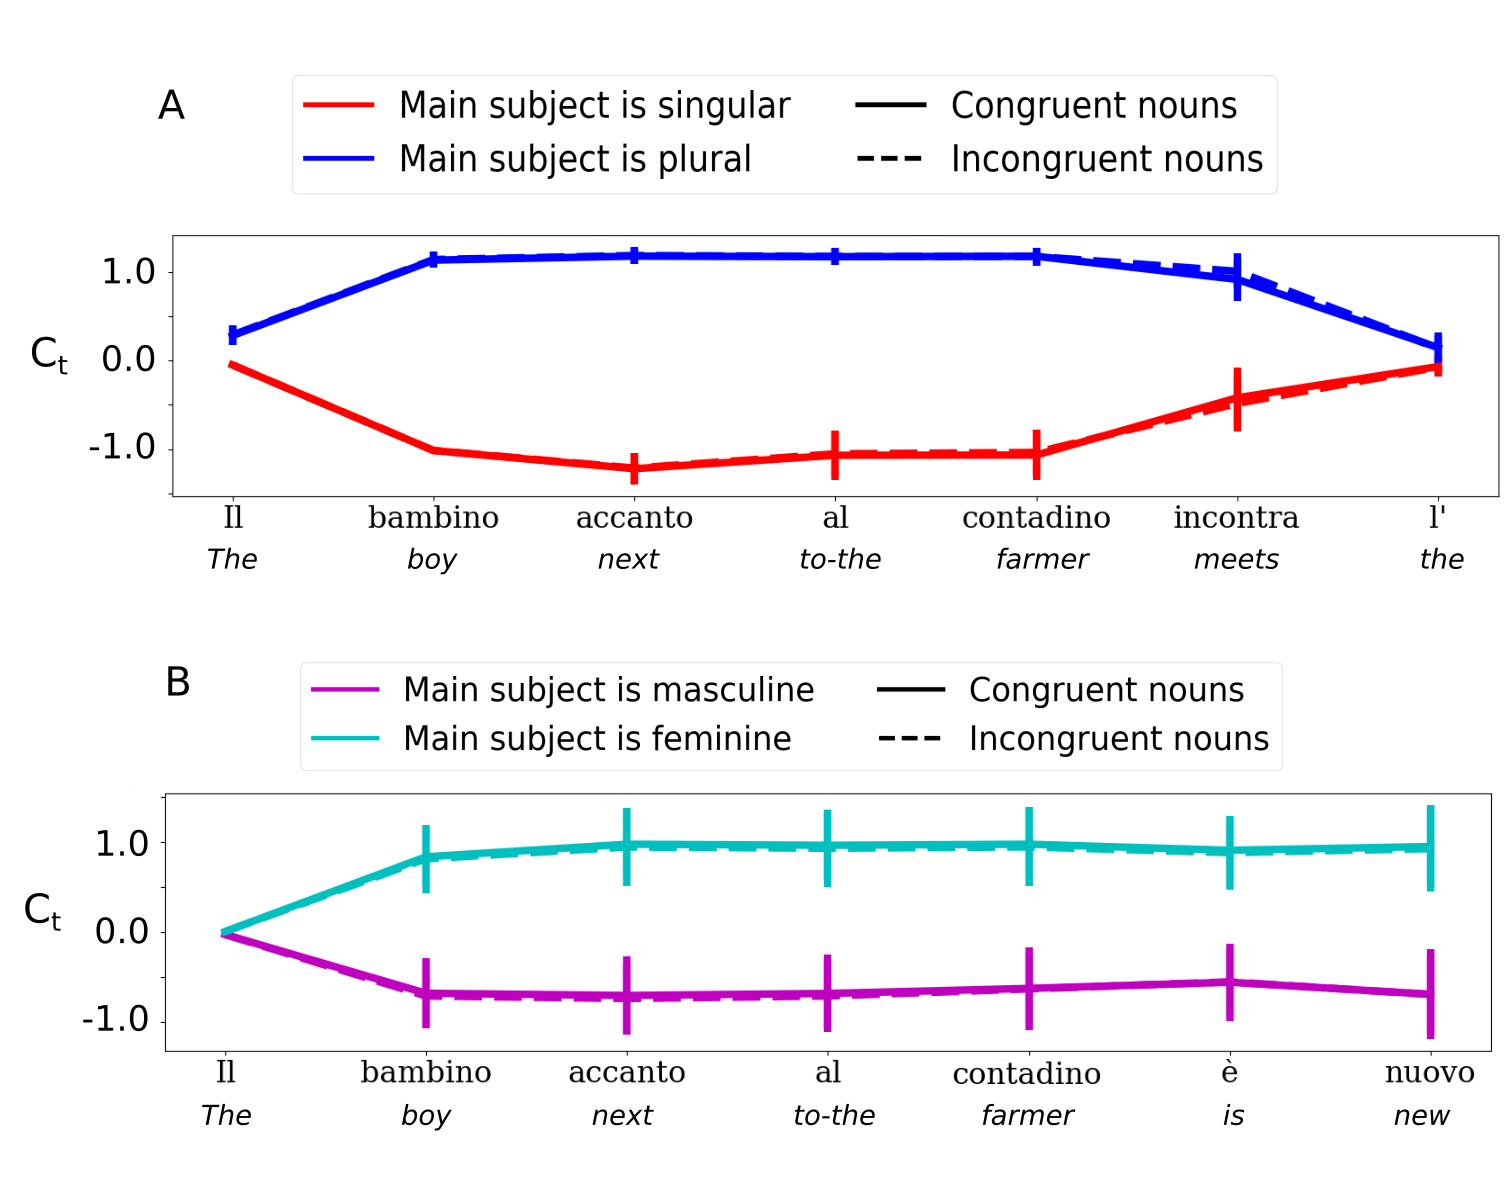
\includegraphics[width=\textwidth]{figures/model_activations_nounpp.png}
    \caption{\textbf{Cell activity of the number unit (panel A) and gender unit (panel B) during the processing of a single long-range dependency across a prepositional phrase.} (A) \textit{Number unit}: four conditions are presented, corresponding to whether the main subject of the sentence is singular (red curves) or plural (blue), and to whether the main subject (`bambino') and the attractor (`contadino') have the same (congruent case; continuous lines) or opposite number (incongruent; dashed). Activity of the number unit depends on the grammatical number of the main subject - positive (negative) for plural (singular) value. Activity is stable throughout the subject-verb dependency, also in the presence of an intervening attractor (dashed lines). (B) \textit{Gender unit}: four conditions corresponding to whether the main subject is masculine (magenta) or feminine (cyan), and to whether the attractor is congruent (continuous) or incongruent (dashed). Activity of the gender unit depends on the gender of the main subject - positive (negative) for feminine (masculine). Activity is stable from the main subject up until the corresponding adjective, also in the presence of an interevning attractor (dashed line).}
    \label{fig:nounpp}
\end{figure} 

\subsubsection{Dynamics of the Number Unit Shows Robustness to Attractors} 
To confirm that unit 815 is a long-range number unit, we visualized the dynamics of the unit during the processing of the long-range dependency, by extracting its activations during the processing of all sentences in the NounPP NA-task. Figure \ref{fig:nounpp}A describes the resulting average cell-state activations. It shows that number information is robustly encoded throughout the subject-verb dependency, also in the presence of an attractor (dashed lines). Furthermore, the dynamics of unit 815 shows that it encodes both singular and plural number, using negative and positive cell activations, respectively. This is different from the English NLM, that developed two separate long-range units specialized on singular and plural respectively.

\subsubsection{Efferent Weights of the Number Unit are Clustered with Respect to Number}
Finally, we extracted the efferent weights of unit 815, which project onto the output layer. Figure \ref{fig:efferent_weights}A shows that unit 815 differentially affects unit activations in the output layer, depending on whether they represent singular or plural forms of the verb. This is consistent with its role as a number unit. In what follows, we therefore refer to unit 815 as the long-range `Number Unit'.

\subsubsection{Short-Range Number Units are also Found in the Network}
As was shown for the English NLM, long-range number units are not the only number-carrying units in the network. `Short-Range' number units also encode grammatical number. However, their activation is not robust to intervening numbers of local attractors. We therefore tested for the presence of short-range number units in the Italian NLM. We found 10 more number units, which encode grammatical number in separate values, and whose efferent weights are clustered with respect to number (Figure \ref{fig:ablation_all_models}).

\subsubsection{Long-Range Gender Units are Also Found in the Network}
For gender, we found one unit that dramatically reduced the performance of the NLM when ablated. Its inner-state dynamics shows robust encoding across the subject-adjective dependency (Figure \ref{fig:nounpp}B), also in the presence of attractors (dashed lines). Connectivity analysis further confirmed that the efferent weights of the long-range `gender' unit are clustered with respect to whether they project to masculine or feminine adjective words in the output layer (Figure \ref{fig:efferent_weights}B).

\vspace{10pt}
In sum, these results replicate and extend previous findings to another language and another grammatical feature. Similarly to English, only a few long-range number units emerged in the Italian NLMs during training. The NLM has developed a similar encoding scheme for both grammatical number and gender, independently. Taken together, this shows that sparse long-range \textit{grammatical-feature} units consistently emerge in NLMs.



